\clearpage
\chapter{Discussion and Conclusion}
\label{chapter:conclusion}

This manuscript reports on several contributions to measuring and reducing software energy consumption.
We used a three-step strategy to lower software energy: benchmarking, measuring, and optimizing.
We started with the benchmarking phase.
Chapter~\ref{chapter:literature_review} discussed the challenges of a successful benchmarking strategy: reproducibility, accuracy, and representativeness.
We concluded that software containers, like "Docker", would be the best fit to ensure that energy studies could be reproduced.
We then extended this reproducibility to an evolving protocol that helps researchers keep up with the rapid pace of software development.
Then, we targeted the accuracy by studying the hardware and software factors that can impact the energy variation and how practitioners can tune them to harness this energy variation.

After establishing a robust benchmarking protocol to create energy-based experiments, we shifted our focus to the optimization side.
We opted to start with Python, the most popular yet energy-hungry programming language.
As a result, we began by examining the energy behavior of Python code in its most common usage.
Then, we presented a non-intrusive method to lessen its energy use.
Following that, we applied the same strategy to another programming language known for its legacy code base, Java, to prove that we can still cut the energy usage of existing running applications without incurring high costs.

Lastly, we used the flexibility of the micro-services architecture to look at how each programming language uses energy in different web scenarios.
We first examined the effects of the various programming languages when dealing with the \emph{Remote Procedure Call} (RPC) protocol.
Then, we extended this study to a more practical application by comparing $261$ web frameworks, each implementing the same website using seven use cases.
Then, we provided practitioners with a dashboard to determine which stack is best for a given situation.


\section{Summary of Contributions}
\label{section:SummaryofContributions}
The contributions reported in this thesis are covered in this section.
The following is a summary of them:

\subsection{Published Papers}
This part summarizes the contributions that have been already accepted in conferences and journals.

\begin{enumerate}
      \item \textbf{Taming energy consumption variations in systems benchmarking}:
            We investigate the phenomenon of variation when measuring the energy consumption of experiments in this study.
            In this paper, we discuss various hardware and software factors that can amplify variations in recorded energy measures, with a focus on the following research questions:
            \begin{description}
                  \item[\textsc{RQ}~1:] Does the benchmarking protocol affect the energy variation?
                  \item[\textsc{RQ}~2:] How important is the impact of the processor features on the energy variation?
                  \item[\textsc{RQ}~3:] What effect does the operating system have on energy variation?
                  \item[\textsc{RQ}~4:] Does the choice of processor make a difference in reducing the energy variation?
            \end{description}

            This contribution shows how processor features can significantly affect the variation in energy use between the benchmarking protocol and the operating system.
            Finally, this study presents several guidelines for controllable parameters that practitioners could easily change to increase the accuracy of their experiments.

            \bibentry{ournani2020taming}


      \item \textbf{Evaluating the impact of Java virtual machines on energy consumption}:
            In this paper, we thoroughly investigate how JVMs affect software energy usage.
            To address the following research concerns, we reveal through this study several trials on hundreds of JVMs versions provided by various providers:
            \begin{description}
                  \item[\textsc{RQ}~1:] What is the impact of existing JVM distributions on the energy consumption of Java-based software services?
                  \item [\textsc{RQ}~1:] What are the relevant JVM settings that can reduce the energy consumption of a given software service?
            \end{description}
            The findings demonstrate that choosing the right JVM platform can significantly reduce energy usage depending on the software and use case.
            This optimization can also be achieved by properly configuring the JIT and GC parameters.

            \bibentry{ournani2021evaluating}
\end{enumerate}

\subsection{Softwares and Tools}
While the benchmarking and optimization parts were presented as chapters in this thesis, the measurement part was primarily based on developing tools that measure the energy consumption for a given use case.
The following is a summary of the tools that were developed during this thesis:
\begin{itemize}
      \item \textbf{Jouleit} (\url{github.com/powerapi-ng/jouleit}): a tool that can be used to monitor energy consumption for any Linux program, this tool was used to compare the energy consumption of different JVMs;
      \item \textbf{JRefferal} (\url{github.com/chakib-belgaid/jreferral}): a tool that allows the user to explore the JVM settings and their impact on the energy consumption of a given Java program. This tool was the result of the second article of this thesis;
      \item \textbf{PyJoules} (\url{pypi.org/project/pyJoules}) is a software toolkit to measure the energy footprint of a host machine along the execution of a piece of Python code. It can measure the energy consumption on the level of script, function, and bloc of code;
      \item \textbf{JouleHunter} (\url{pypi.org/project/joulehunter}): an energy profiler for python applications. It can be used to highlight the functions that consume the most energy in a given Python program. Its main usage is to help developers do an exploratory analysis of their application to scope the functions that should be optimized to be then targeted by PyJoules;
      \item \textbf{GreenBoard} (\url{github.com/chakib-belgaid/greenboard}): a dashboard designed to help developers choose the best stack for their web application. It is based on the results of the third article of the last chapter.
\end{itemize}



\subsection{Future Submissions}
\begin{itemize}
      \item Reducing the energy consumption of Python using non-intrusive techniques,
      \item Empirical analysis on the energy consumption of different web frameworks,
      \item The impact of programming languages on energy consumption of web services (a case study of RPC protocol),
      \item How do ORMs affect how much energy is used? A case study of Django.
\end{itemize}

\section{Future Work\note{ In Draft }}
While our contributions are a good start to the energy-aware software engineering field, there are still many challenges to overcome.
This is just the tip of the iceberg.
The following perspectives are some of the challenges that we would like to address in the future.

\subsection{Short-Term Challenges}
Before starting a journey looking for a new mine, one should first look at the available resources.
In the same way, we need to first look at the resources available to us before we start looking for new challenges.
The following are some of the challenges that we can address in the short term.

\paragraph{Studying the evolution of Python interpreters.}
In Chapter~\ref{chapter:python}, we compared several python interpreters.
However, most of these alternative solutions were based on Python\,2, which is now deprecated.
On the other hand, the default python interpreter (aka CPython) has included many features and optimization since our last study, such as the introduction of Python introduced the \texttt{dataclasses} in version 3.7 (PEP~557)\footnote{\url{https://peps.python.org/pep-0557/}} that can be used to reduce the memory footprint of Python objects, the new parser in Python\,3.9,\footnote{\url{https://docs.python.org/3/whatsnew/3.9.html}} the user type alias in Python\,3.10.\footnote{\url{https://peps.python.org/pep-0613/}}
And, the most interesting changes for us occurred in CPython 3.11, which is claimed to be 25\% faster than Python\,3.10.\footnote{\url{https://github.com/faster-cpython/ideas}}.
We need to re-evaluate the impact of these changes on the energy consumption of Python programs.

\paragraph{Studying the impact of ORMs.}
We continue with our work with Python, and this time we will dive deeper into the impact of the ORMs.
As shown in Section~\ref{sec:webdev}, the ORMs are the most energy-consuming part of a web application.
We intend to widen this analysis to other Python ORMs, such as \textsc{SQLAlchemy}\link{https://www.sqlalchemy.org/} and \textsc{Peewee}.\link{http://docs.peewee-orm.com/en/latest/}
We will also explore the real relationship between the ORM, the database, and the web framework.

\paragraph{Studying the impact of Machine learning.}
In Chapter~\ref{chapter:python}, we showed that training accuracy has a huge cost on the energy using a single model.
However, in practice, we often use multiple models to address a given problem.
We will explore the impact of using multiple models on the energy consumption of a machine learning application, as well as compare the energy consumption of different machine learning frameworks, such as \textsc{PyTorch},\link{https://pytorch.org/} \textsc{SciKit-Learn},\link{https://scikit-learn.org/stable/} and \textsc{TensorFlow}.\link{https://www.tensorflow.org/}



\paragraph{Studying the impact of JVM bytecode.}
As we have seen in Chapter~\ref{chapter:java}, the choice of the JVM can greatly impact the energy consumption of hosted applications.
On the other hand, we have seen in Chapter~\ref{chapter:porgramming_langauges} that other JVM-based languages depicted half power consumption of the Java code.
Was it only because of the adopted web framework?
Or is there a real difference between the JVMs and the bytecode handled by JVM-based languages?
We will explore this question by comparing the energy consumption of different JVMs and JVM-based languages, such as Scala, Kotlin, Groovy, and Clojure.

\paragraph{Revisiting the impact of programming languages.}
One of the hardest challenges when comparing the energy consumption of multiple programming languages was the bias of the expertise of the programmer.
One solution was to create a reference benchmark that allows one to compare several programming languages.\link{https://benchmarksgame-team.pages.debian.net/benchmarksgame/index.html}
This benchmark has been adopted by many researchers, such as the work of \citeauthor{couto2017towards}~\cite{couto2017towards}, while others were to use some basic algorithms, like \cite{noureddine_preliminary_2012} who compare the energy consumption using the Hanoi tower problem\link{https://en.wikipedia.org/wiki/Tower_of_Hanoi} using different programming languages, or even simpler benchmarks, like the Rosettacode base.\link{https://rosettacode.org/wiki/Rosetta_Code}
However, this scope is limited to single algorithms and does not help to cover production-like conditions, this is why we shifted to the web frameworks.
Nonetheless, semantic analyzers issued from the OpenAI project\link{https://openai.com/} like the automatic test generator \textsc{Ponicode}\link{https://www.ponicode.com/} and AI code generator,\link{https://github.com/features/copilot} an interesting new feature provided by the GitHub copilot is GitHub copilot labs\link{https://githubnext.com/projects/copilot-labs/} is the ability to automatically translate the code from one language to another.
We will explore the impact of this feature on the energy consumption of a program.


\paragraph{raising awareness of the energy consumption of the Softwares}
While this thesis's main focus was to optimize energy consumption using comparative studies, it was easier to say that approach \texttt{X} is greener than approach \texttt{Y}, no matter which metric we were using.
However, it will not be the case for developers when measuring the energy consumption of their programs.
Some tried to give labels, such as (A,B,C\dots), while others translated these raw metrics in an equivalent of fuel consumption (e.g., 1 liter of fuel per 1000 lines of code).
Most of the approaches were to use the carbon emission, such as~\cite{patterson2021carbon} or ecograder~\link{https://ecograder.com/} as a pivot metrics to quantify the environmental cost of osftware.
We intend to explore these approaches and study how they can be used to increase awareness of the energy consumption of their code.



\subsection*{Representativeness}:
As reported in the state of the art, a successful benchmark meets three criteria: reproducibility, accuracy, and representativeness.
This Ph.D. thesis mostly discussed two of these criteria: reproducibility, and accuracy.
However, we did not discuss the representativeness of our benchmarks.
We relied on state-of-the-art benchmarks to represent real-world applications.
Nevertheless, the gap between these benchmarks and the industry is getting bigger and bigger, due to the extreme pace of software development.
In the future, we would like to tackle the issue of representativeness and discuss how we can improve our protocol to fit real-world applications.
After all, what is the purpose of doing optimizations if they cannot be applied to real-world applications?

First, we will consider taking advantage of the popularity of CI/CD among developers to provide some insights into the energy consumption of their code.
We did prototype a sonar tool that can report on the energy consumption of Java-based code repository.
Figure~\ref{fig:JunitSonarplugin} shows the work of our intern who used a Sonar plugin to highlight the energy evolution of Java applications over time.
This prototype got even more sophisticated to become Joule-dff\link{https://github.com/davidson-consulting/diff-jjoules}, which is a tool to be added in continuous integration to highlight the energy evolution of the Java programs.
We intend to push this even further to detect the commits responsible for an increase or the optimization within the source code.
\begin{figure}[!h]
      \centering
      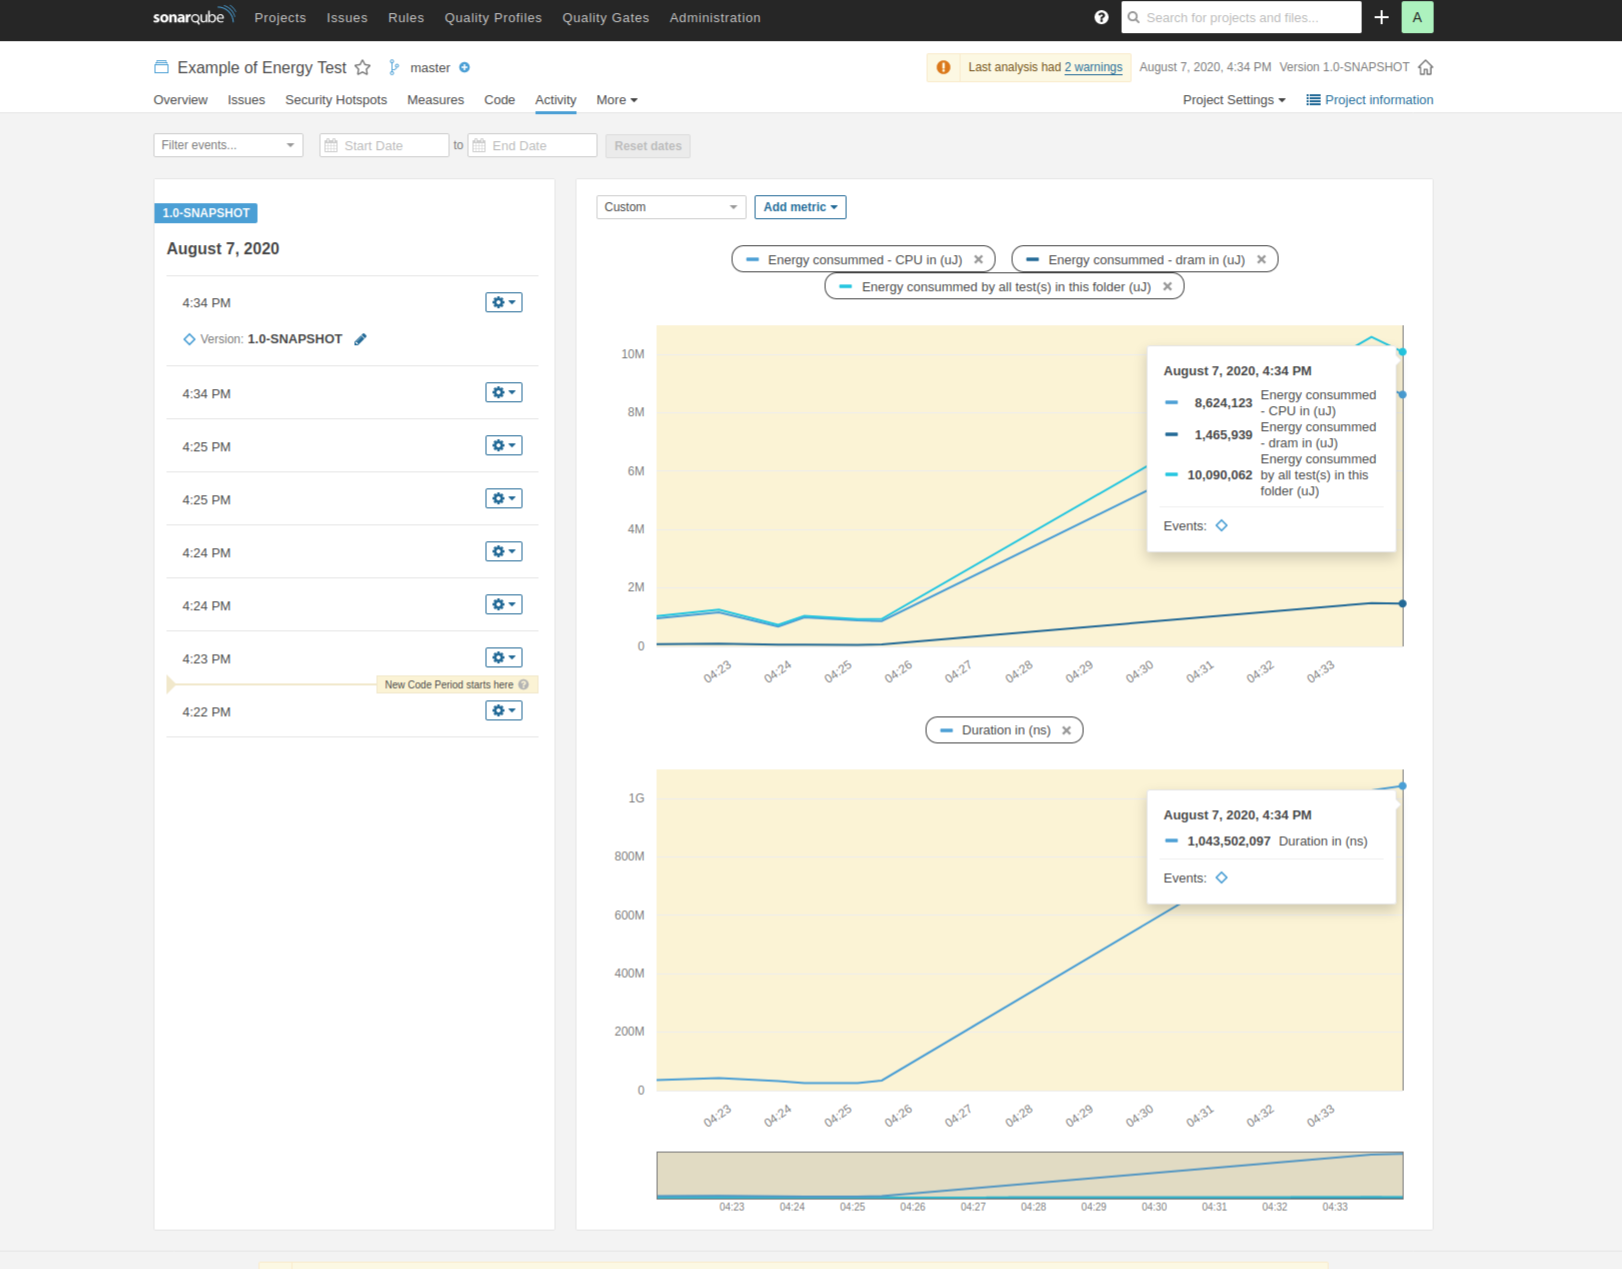
\includegraphics[width=0.8\linewidth]{chapters/JunitSonarplugin}
      \caption{Sonar Energy plugin for JUnit}
      \label{fig:JunitSonarplugin}
\end{figure}


\subsubsection{Energy impact vs Energy consumption}
To make the software more eco-friendly, both state-of-the-art and this thesis focused on reducing software energy consumption. To accomplish this, we sought to isolate the energy consumption of the software under test as much as possible, primarily by running the tests on an isolated machine that runs only a few services. Others tried to infer the energy consumption of a single process using additional metrics that vary from the CPU usage, such as \cite{noureddine-issta-2016} to more sophisticated models like~\cite{fieni2020smartwatts,fieni2021selfwatts}.

However, by the end of this thesis, I realized that isolating the energy consumption by running the tests on an isolated machine does not represent real-world conditions; many processes are running in parallel. On the other hand, our benchmark can compete with other processes for resources such as CPU, memory, and network. Therefore, this program can increase the energy consumption of other processes running on the same machine, although its energy consumption is low.

This is why I've started to work on a new project called \textsc{Energy Impact} that aims to measure the energy impact of software.
According to the work of \citeauthor{barroso2007case}~\cite{barroso2007case}, servers operate most of the time at between 10 and 50 percent of their maximum utilization levels. Moreover, as shown in Figure~\ref{fig:soa_energy_efficiency} with 50\% of the servers' capacity, the server operates only with  75\% of its maximum power. In other words, it will cost us only 25\% of the energy to operate the extra 50\% of the servers' capacity.

\begin{figure}[!h]
      \centering
      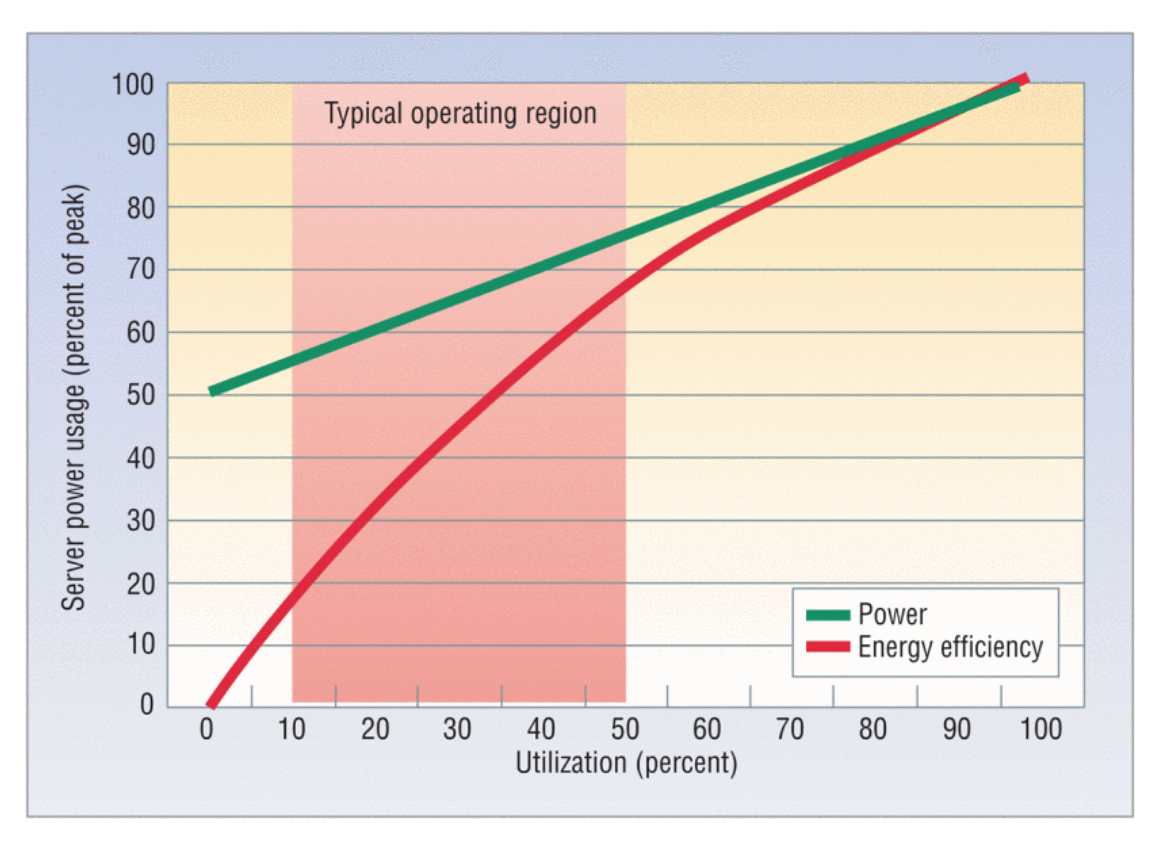
\includegraphics[width=0.9\linewidth,keepaspectratio]{chapters/soa_energy_efficiency}
      \caption{Power efficiency vs power consumption\cite{barroso2007case}}
      \label{fig:soa_energy_efficiency}
\end{figure}

\begin{figure}[!h]
      \centering
      \caption{Evolution of CPU power}
      \label{fig:power_evolution_greenfaas}
      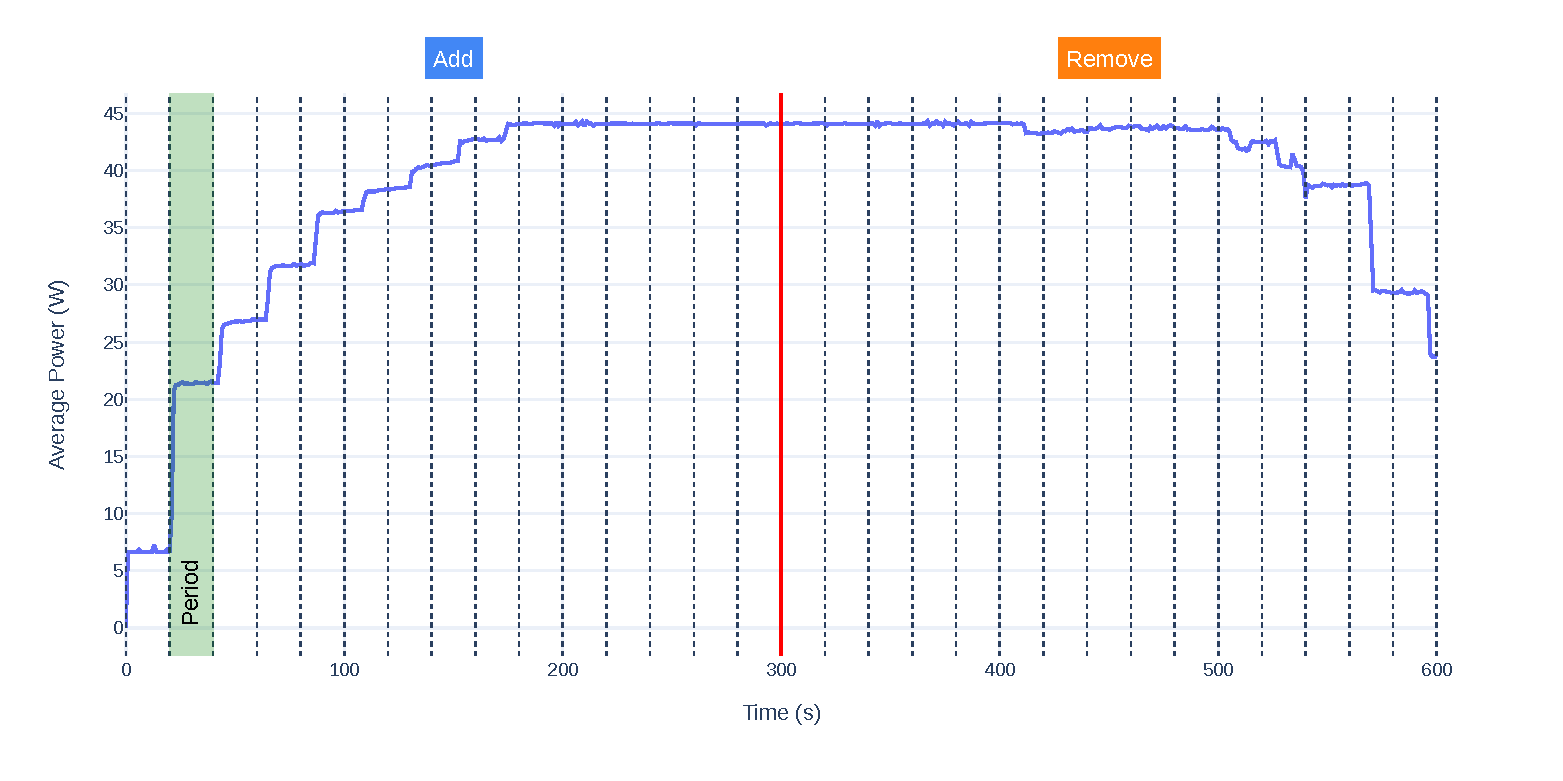
\includegraphics[width=\linewidth]{chapters/power_evolution_greenfaas}
\end{figure}

In order to confirm whether this hypothesis still holds. We run the following experiment.
First, we took a machine with minimal services, then created a process that stresses one core by doing some mathematical operations, and each second we introduced a copy of this process. after a while, we removed these copies one by one.
Figure~\ref{fig:power_evolution_greenfaas} displays the machine's power consumption during this experiment. As one can notice, the introduction of the first copies had a greater cost than the other ones, despite not sharing the same core. And the more we approach the peak of power, the less significance the introduction of a new process has on power consumption to be almost zero after the 9th copy.

One should note that this experiment was conducted on a machine with the following configuration:
Intel(R) Core(TM) i7-3740QM CPU @ 2.70GHz, with 4 physical cores and 4 hyper threads, 16GB RAM, and 687GB HDD.
Therefore with the introduction of the eighth copy, we have already saturated the machine's capacity, and the introduction of the ninth copy had no impact on the power consumption.
\begin{figure}[!h]
      \centering
      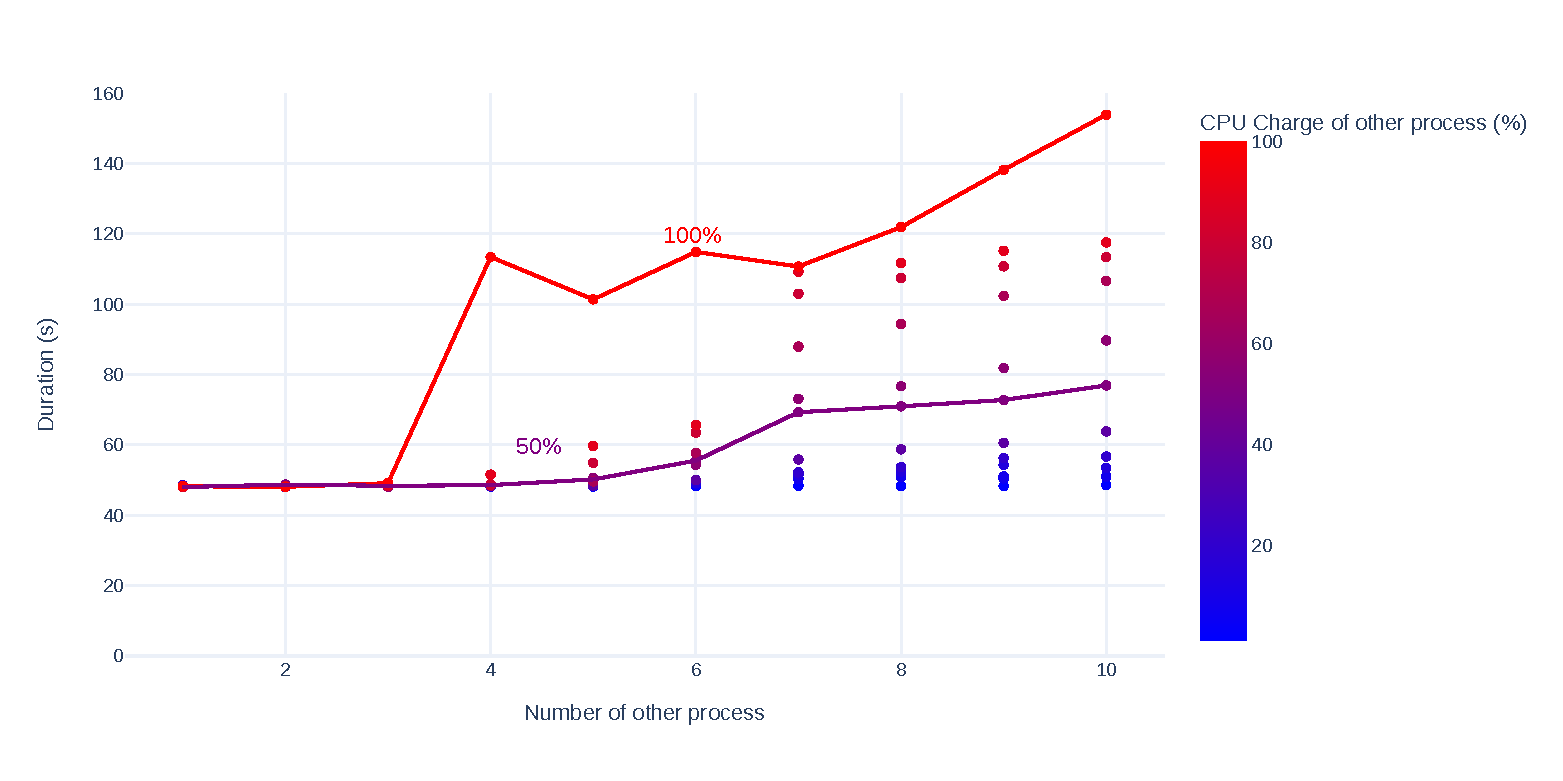
\includegraphics[width=\linewidth]{chapters/green_faas_duration}
      \caption{Evolution of CPU behavior during multiple contexts }
      \label{fig:green_faas_duration}
\end{figure}

To push this experiment further, we created a stressing tool that allows us to fix the number of cores and \% usage of each core to simulate a production context. we then run a benchmark( graph coloration algrothim\link{https://github.com/chakib-belgaid/lazy-green-code-test/tree/master/exp01}) using multiple configurations.
Figure~\ref{fig:green_faas_duration} displays the overall performance of the benchmark. As one can see, the execution time remained the same when the context was using 3 cores at any saturation level,
this is because we have 4 physical CPU cores, therefore each process was running a different core,(3 cores were used by the context and the other one was used by the benchmark). However, behavior changes when the context consumes more than 3 cores. CPU saturation tends to have a great impact on the performance of the benchmark. when the benchmark was using a hyper thread of the same core as one of the context workers it took almost double the time to finish the same job.
As when we saturated only 50\% of the CPU capacity, this increase didn't happen until the context used 7 cores, and in the worst-case scenario ( 10 extra processes) it took only 75 seconds to finish the job.

\begin{figure}[!h]
      \centering
      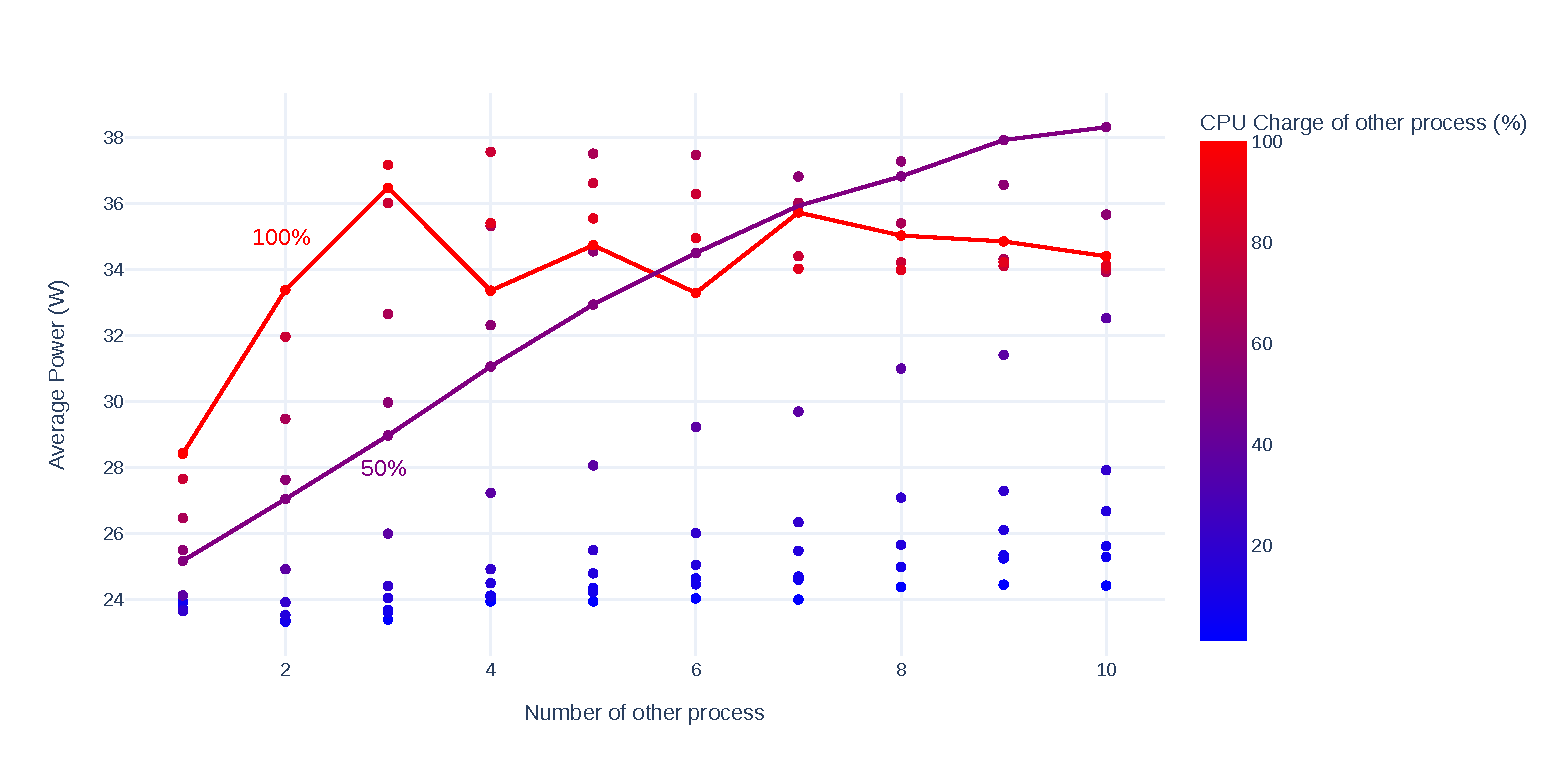
\includegraphics[width=\linewidth]{chapters/green_faas_power}
      \caption{Evolution of CPU behavior during multiple contexts }
      \label{fig:green_faas_power}
\end{figure}

On the other hand, as we can see in Figure~\ref{fig:green_faas_power}, the average power behavior of the system had different behavior. With the 100\% saturation scenario, the power consumption hit its peak as soon as we hit the 4 core usage 3 from the context and 1 from the benchmark), and it kept fluctuating until the 8th core saturation, after that it was in a constant decrease. This was because the processes were competing with each other for cache usage, which led to a significant number of cache defaults that slowed down the CPU frequency which led to a decrease in power consumption.

However, when we used 50\% of the CPU capacity, the power kept increasing by adding the number of extra processes. As for the scenarios where we used more than 50\% of the CPU capacity, the power consumption kept increasing until it hit its peak then it start to decrease; this number of processes needed to reach the peak varies according to the saturation level.





\begin{figure}[!h]
      \centering
      \caption{Evolution of CPU behavior during multiple contexts }
      \label{fig:green_faas_energy}
      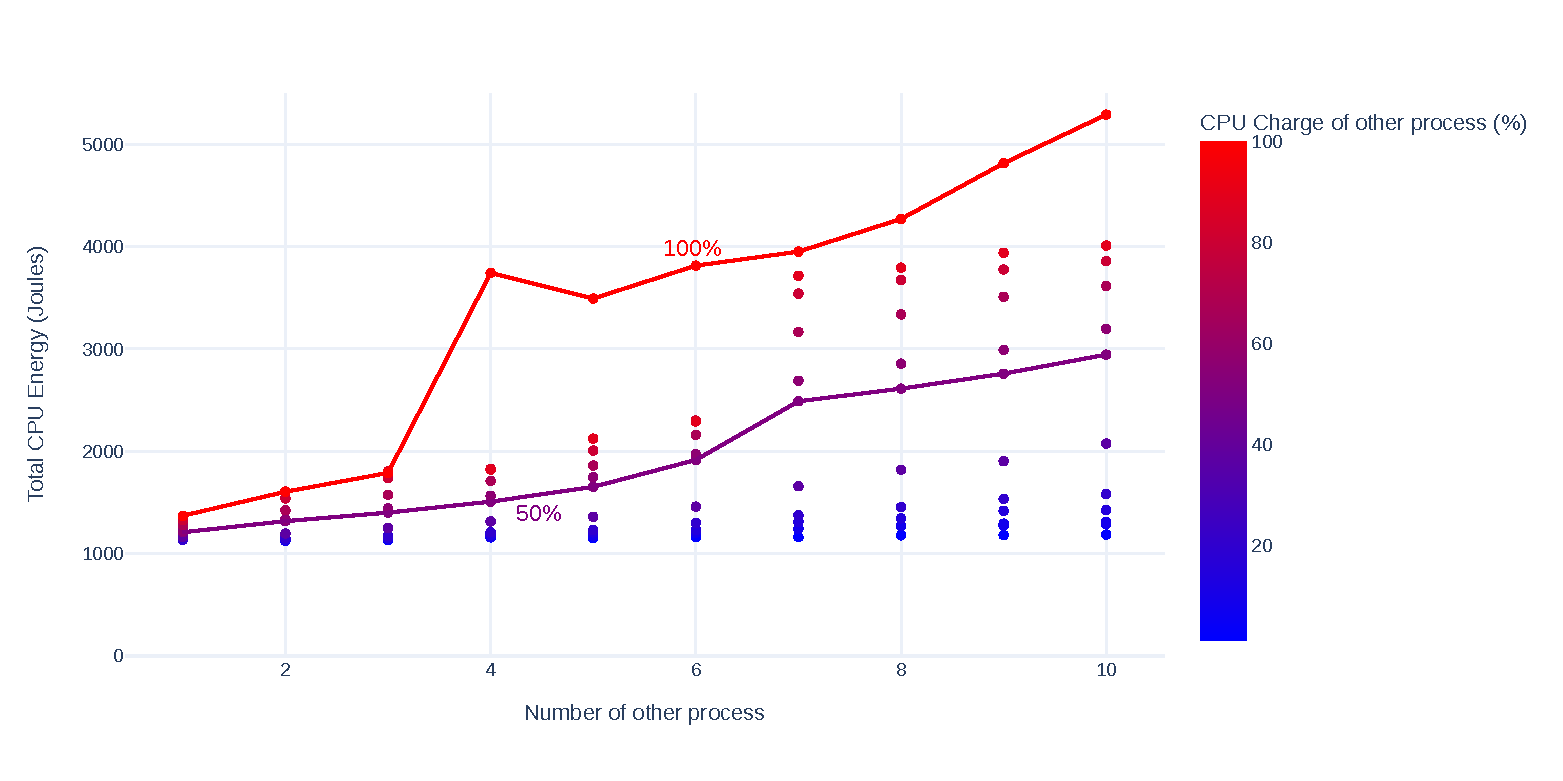
\includegraphics[width=\linewidth]{chapters/green_faas_energy}
\end{figure}

On the other hand, as shown in Figure~\ref{fig:green_faas_energy} the energy started increasing from the beginning, this is due to an increase in power that we will discuss










\begin{figure}[!h]
      \centering
      \caption{Evolution of CPU behavior during multiple contexts }
      \label{fig:green_faas_impact}
      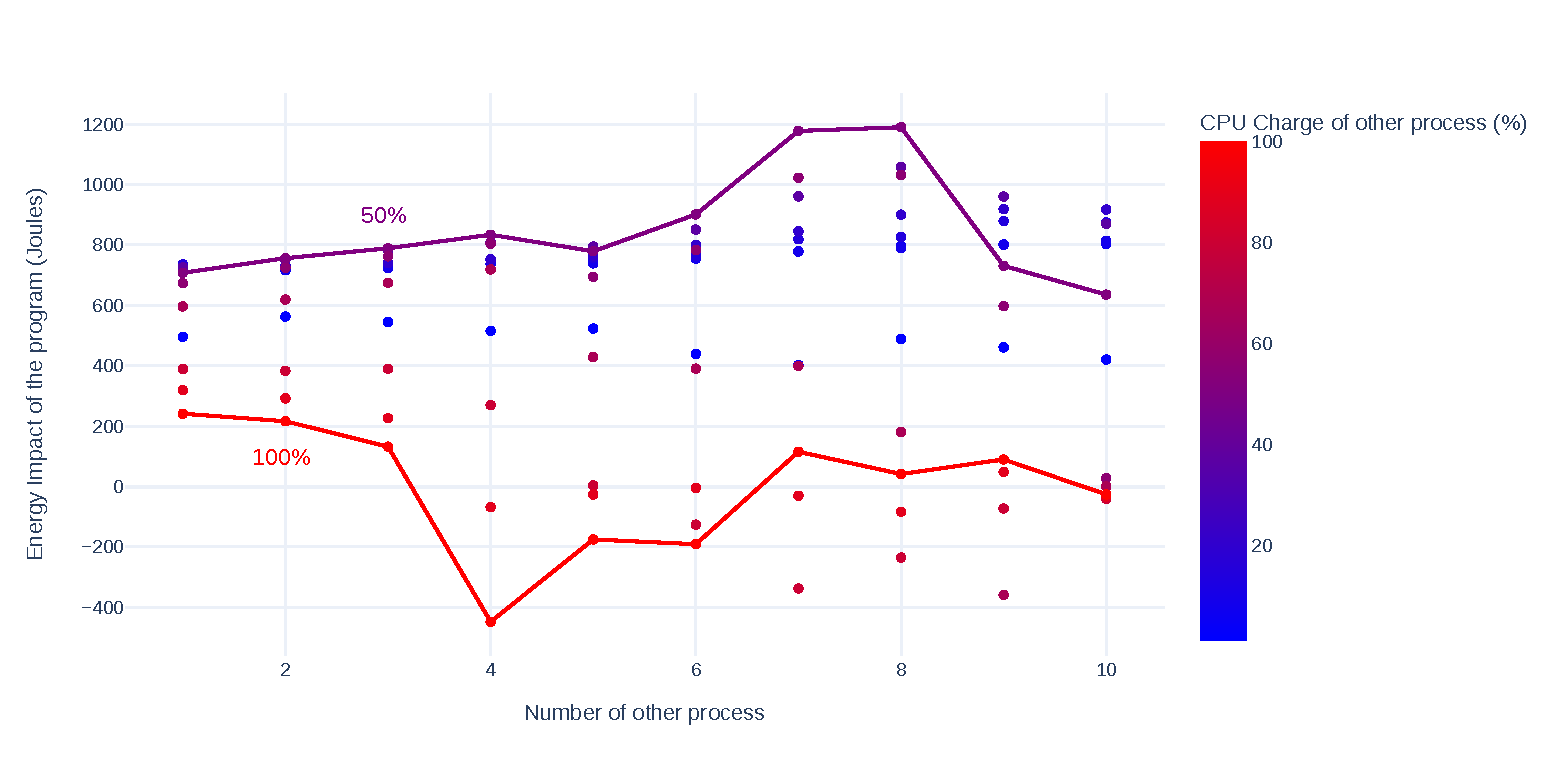
\includegraphics[width=\linewidth]{chapters/green_faas_impact}
\end{figure}



\url{https://github.com/chakib-belgaid/lazy-green-code-test}



\begin{enumerate}
      \item lazy code, sacrificing the performance to get a better energy consumption --> green faas
      \item more representative benchmarks, using several CPU saturation levels
      \item measuring the energy impact instead of the row energy consumption. ( the highway analogy when a single application consumes less energy, however the total energy consumption of the system increases )
\end{enumerate}
\vfill \strut  % to fill the rest of the page with blank lines
\cleardoublepage